% Data flow diagram
% Author: David Fokkema
\documentclass{standalone}
\usepackage{tikz}
\usetikzlibrary{arrows,quotes,shapes.multipart,arrows.meta,matrix,shapes.geometric,backgrounds}

% Defines a `datastore' shape for use in DFDs.  This inherits from a
% rectangle and only draws two horizontal lines.
\makeatletter
\pgfdeclareshape{datastore}{
  \inheritsavedanchors[from=rectangle]
  \inheritanchorborder[from=rectangle]
  \inheritanchor[from=rectangle]{center}
  \inheritanchor[from=rectangle]{base}
  \inheritanchor[from=rectangle]{north}
  \inheritanchor[from=rectangle]{north east}
  \inheritanchor[from=rectangle]{east}
  \inheritanchor[from=rectangle]{south east}
  \inheritanchor[from=rectangle]{south}
  \inheritanchor[from=rectangle]{south west}
  \inheritanchor[from=rectangle]{west}
  \inheritanchor[from=rectangle]{north west}
  \backgroundpath{
    %  store lower right in xa/ya and upper right in xb/yb
    \pgfset{outer xsep=1.5cm}
    \pgfset{outer ysep=1.5cm}
    \southwest \pgf@xa=\pgf@x \pgf@ya=\pgf@y
    \northeast \pgf@xb=\pgf@x \pgf@yb=\pgf@y
    \pgfpathmoveto{\pgfpoint{\pgf@xa}{\pgf@ya}}
    \pgfpathlineto{\pgfpoint{\pgf@xb}{\pgf@ya}}
    \pgfpathmoveto{\pgfpoint{\pgf@xa}{\pgf@yb}}
    \pgfpathlineto{\pgfpoint{\pgf@xb}{\pgf@yb}}
 }
}
\makeatother

\tikzset{
  database_plate/.style={
    cylinder,draw,rotate=90,minimum width=1.5cm,path picture=
    {
      \draw (path picture bounding box.160) to[out=180,in=180,looseness=0.3] (path picture bounding box.20);
      \draw (path picture bounding box.200) to[out=180,in=180,looseness=0.3] (path picture bounding box.340);
    }
  },
  database/.style={
    cylinder,shading=axis,shading angle=0,top color=yellow!10,bottom color=yellow!60,draw,rotate=90,minimum width=1.5cm
  }
}

\begin{document}
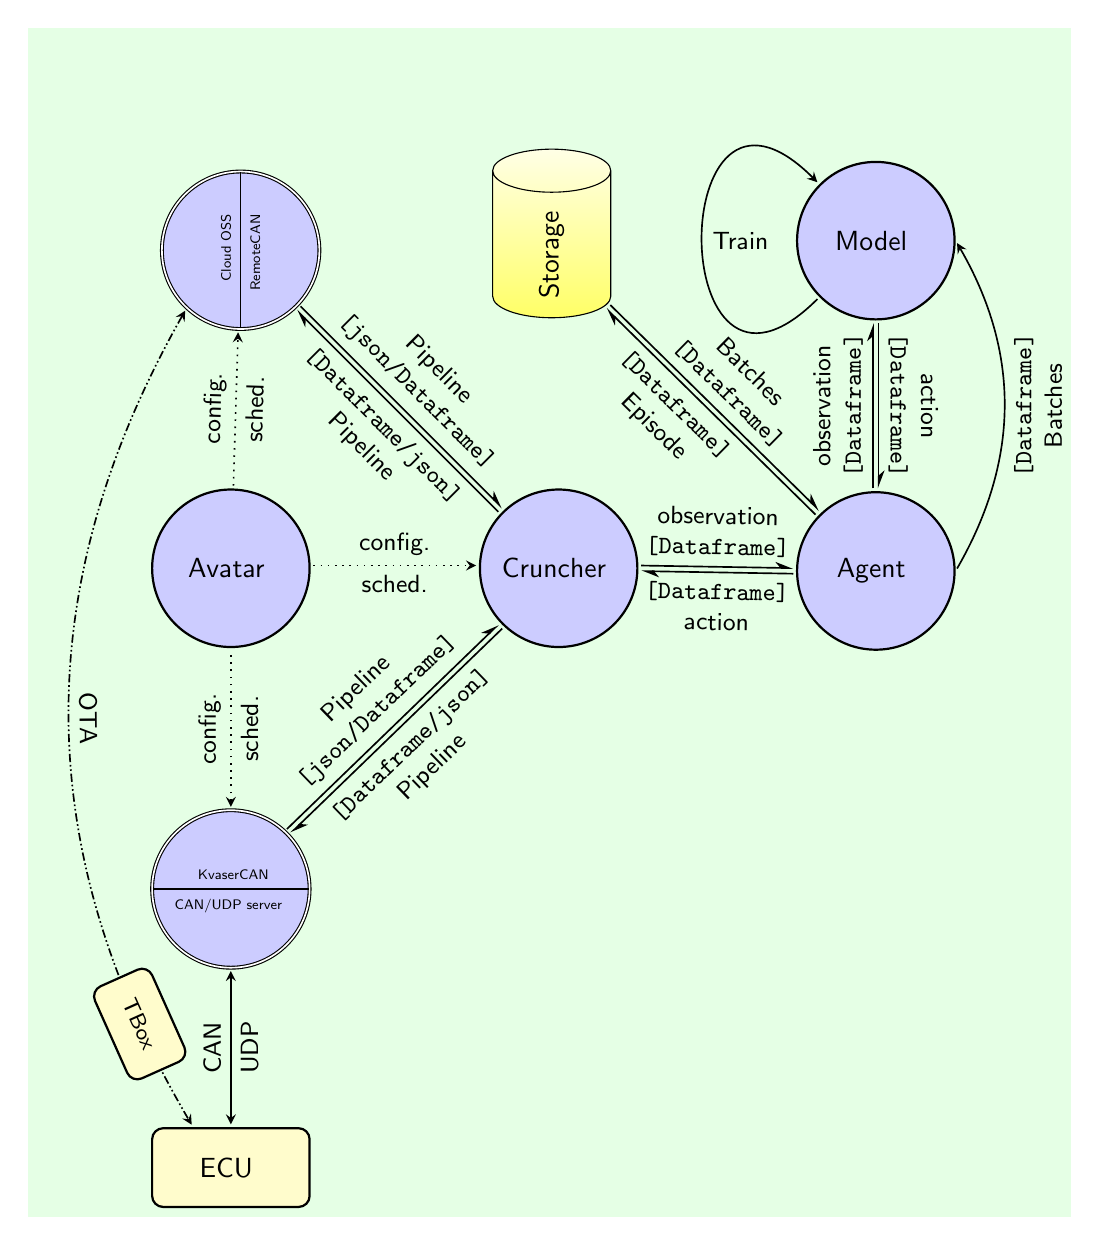
\begin{tikzpicture}[
  font=\sffamily,
  every matrix/.style={ampersand replacement=\&,column sep=2cm,row sep=2cm},
  hw/.style={draw,thick,minimum width=2cm,minimum height=1cm,rounded corners,fill=yellow!20,inner sep=.3cm},
  process/.style={draw,thick,circle,fill=blue!20},
  multimodal/.style={circle split,draw,double,fill=blue!20,font=\sffamily\tiny},
  sink/.style={hw,fill=green!20},
  datastore/.style={draw,very thick,shape=datastore,inner sep=.3cm},
  dots/.style={gray,scale=2},
  to/.style={->,>=stealth',shorten >=1pt,semithick,font=\sffamily\footnotesize},
  every edge/.style={draw,>=stealth,shorten <=1pt, shorten >=1pt,semithick,font=\sffamily\footnotesize},
  every edge quotes/.style={auto=left,sloped,font=\sffamily\small},
  every node/.style={align=center}
]
  %every edge/.style={->,>=stealth',shorten >=1pt,semithick,font=\sffamily\footnotesize},
  % Fill the background


  % Position the nodes using a matrix layout
  \matrix (m) [matrix of nodes,
      row sep = 2em, column sep = 2em,
      minimum size=2cm]{
    |[multimodal,rotate=90] (cl)| {
      Cloud OSS \nodepart{lower}
    } RemoteCAN
    \& |[database] (db)| {Storage}
    \& |[process] (mo)| {Model} \\
    |[process] (av)| {Avatar}
    \& |[process] (cr)| {Cruncher}
    \& |[process] (ag)| {Agent} \\
    |[multimodal] (kv)| {
      KvaserCAN
      \nodepart{lower}
    } CAN/UDP server
    \&
    \& \\
    |[hw] (v)| {ECU} \&  \&\\
  };

  % Draw the arrows between the nodes and label them.
  \draw (cr.2) edge [arrows={-Stealth[harpoon]},"observation\\\texttt{\string[Dataframe\string]}",midway,align=center] (ag.178)
        (ag.182) edge [arrows={-Stealth[harpoon]},"\texttt{\string[Dataframe\string]}\\action"',midway,align=center] (cr.358);
  \draw (kv.47) edge [arrows={-Stealth[harpoon]},"Pipeline\\\texttt{\string[json/Dataframe\string]}",midway,align=center] (cr.223)
        (cr.227) edge [arrows={-Stealth[harpoon]},"\texttt{\string[Dataframe/json\string]}\\Pipeline"',midway,align=center] (kv.43);
  \draw (cl.227) edge [arrows={-Stealth[harpoon]},"Pipeline\\\texttt{\string[json/Dataframe\string]}",midway,align=center] (cr.133)
        (cr.137) edge [arrows={-Stealth[harpoon]},"\texttt{\string[Dataframe/json\string]}\\Pipeline"',midway,align=center] (cl.223);
  \draw (db.227) edge [arrows={-Stealth[harpoon]},"Batches\\\texttt{\string[Dataframe\string]}",midway,align=center] (ag.133)
        (ag.137) edge [arrows={-Stealth[harpoon]},"\texttt{\string[Dataframe\string]}\\Episode"',midway,align=center,pos=0.6] (db.223);
  \draw (ag.92) edge [arrows={-Stealth[harpoon]},"observation\\\texttt{\string[Dataframe\string]}",midway,align=center] (mo.268)
        (mo.272) edge [arrows={-Stealth[harpoon]},"action\\\texttt{\string[Dataframe\string]}",midway,align=center] (ag.88);
  \draw (ag.0) edge [->,bend right,"\texttt{\string[Dataframe\string]}\\Batches"',midway,align=center] (mo.0);
  \draw (mo) edge[->,loop left,out=225,in=135, looseness=5] node[font=\sffamily\small,right]{Train} (mo);
  \draw (av.2) edge [->,dotted,"config." above,"sched." below,font=\sffamily\tiny] (cr.178);
  \draw (kv) edge [<-,dotted,"config." above,"sched." below,font=\sffamily\tiny] (av);
  \draw (av) edge [->,dotted,"config." above,"sched." below,font=\sffamily\tiny] (cl);
  \draw (v) edge [<->,"CAN" above, "UDP" below] (kv);
  \draw (cl.137) edge [<->, densely dash dot dot,bend right,"OTA"] node[hw,minimum width=1cm,minimum height=0.5cm,solid,very near end, sloped,]{TBox} (v.133);

  % Background rectangle
    \begin{scope}[on background layer]
        \fill[green!10] (current bounding box.south west) rectangle (current bounding box.north east);
    \end{scope}
\end{tikzpicture}
\end{document}
